%%%%%%%%%%%%%%%%%%%%%%%%%%%%%%%%%%%%%%%%%%%%%%%%%%%%%%%%%%%%%%%%%%%%%%%%%%%%%%%%%
%																				%
%	TRABAJO:	Trabajo Final													%
%				Especialidad en Ingenier�a en Sistemas de Informaci�n			%
%																				%
%		Titulo:																	%
%																				%
%		Autor:	Juli�n Nonino													%
%																				%
%	Capitulo sobre el software desarrollado										%	
%																				%
%	A�o: 2016																	%
%																				%
%%%%%%%%%%%%%%%%%%%%%%%%%%%%%%%%%%%%%%%%%%%%%%%%%%%%%%%%%%%%%%%%%%%%%%%%%%%%%%%%%

\chapter{Aplicaciones Desarrolladas}
\label{chapter_aplicaciones_desarrolladas}

En �ste cap�tulo se mostrar�n las aplicaciones desarrolladas para hacer uso del
sistema de procesamiento de datos presentado en secciones
anteriores (\ref{arquitectura_general}).

Los datos ingresan al sistema a trav�s de Apache Kafka, por ello, se comenz�
generando una aplicaci�n para enviar datos al servicio de Apache Kafka y otra
para consumirlos directmente desde Apache Kafka.

Tambi�n, se desarrollo una aplicaci�n de Apache Storm, \textbf{topolog�a}, que
recuperar� los datos del servicio de Apache Kafka teniendolos disponibles para
procesarlos en Apache Storm.

\section{Productor de Datos de Kafka}
\label{productor_kafka}

	Para generar una entrada de datos al sistema, se implement� una aplicaci�n Java
	encargada de publicar datos en Apacker Kafka. Paralelamente, se implement� una
	aplicaci�n consumidora de datos con el objetivo de comprobar que la producci�n
	de datos es correcta.

	\begin{figure}[H]
		\centering
		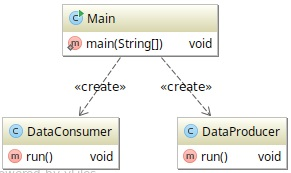
\includegraphics[width=.6\linewidth]{./informe/desarrollo/img/KafkaClassDiagram}
	\end{figure}

	Existe una clase \emph{Main} encargada de recibir los par�metros de entrada de
	la aplicaci�n e inicializar hilos de ejecuci�n productores y/o consumidores de
	datos seg�n sea necesario.

	\lstinputlisting[language=Java,
					 caption={Clase Main de la aplicaci�n de Apache Kafka},
					 label=kafka_app_main
					]{./software/kafka/src/main/java/ar/edu/utn/frc/posgrado/jnonino/kafka/Main.java}
	
	Como par�metros, se reciben la lista de brokers de Apache Kafka,
	indicadores \emph{yes|no} para habilitar el hilo productor y/o el hilo
	consumidor y finalmente, un par�metro n�merico indicando, en milisegundos, la
	tasa de producci�n de mensajes.

	\newpage

	La producci�n de datos se hacer en una clase llamada
	DataProducer (\ref{kafka_app_producer}) que extiende de la clase \emph{Thread}
	de Java. Al momento de instanciar un objeto de �sta clase, se debe enviar la
	lista de brokers de Kafka y el valor de milisegundos que indica la tasa de
	producci�n de mensajes.

	\lstinputlisting[language=Java,
					 caption={Productor de datos de la aplicaci�n de Apache Kafka},
					 label=kafka_app_producer
					]{./software/kafka/src/main/java/ar/edu/utn/frc/posgrado/jnonino/kafka/DataProducer.java}

	El m�todo \emph{run} lee datos desde un archivo texto donde cada l�nea es un
	mensaje independiente y los publica en Apache Kafka. El formato de los
	mensajes incluye pais, provincia, ciudad, tiempo, temperatura, humedad,
	presi�n, velocidad y direcci�n del viento.
	
\lstset{language=Bash}
\begin{lstlisting}
Argentina,Catamarca,Aconquija,1207105200000,25.2,49.7,962,5.1,SUR
\end{lstlisting}

	\newpage
	
	Para el caso del consumidor de datos, se repite el mismo esquema de instanciar
	un objeto que extiende la clase \emph{Thread} de Java recibiendo como par�metro
	la lista de brokers de Kafka.
	
	En el m�todo \emph{run}, se recuperan mensajes desde el servidor y se los
	imprimi en la consola de usuario.

	\lstinputlisting[language=Java,
					 caption={Consumidor de prueba de la aplicaci�n de Apache Kafka},
					 label=kafka_app_consumer
					]{./software/kafka/src/main/java/ar/edu/utn/frc/posgrado/jnonino/kafka/DataConsumer.java}

\section{Topolog�a de Procesamiento de Datos de Storm}
\label{topologia_storm}
	
	\begin{figure}[H]
		\centering
		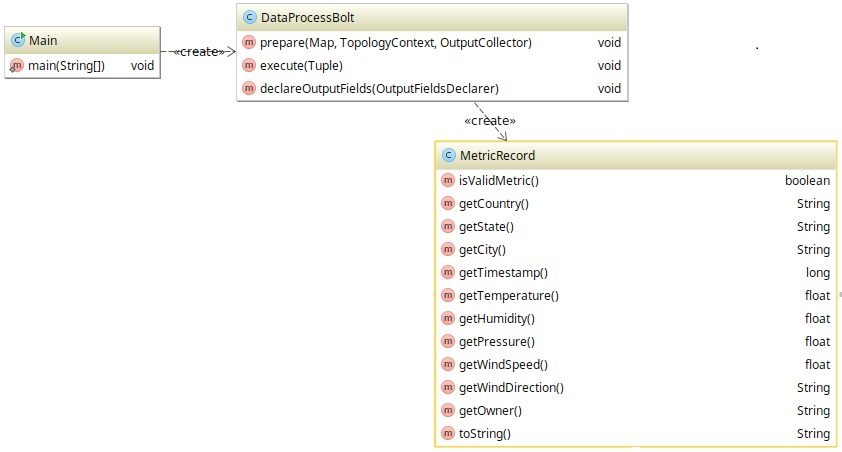
\includegraphics[width=1\linewidth]{./informe/desarrollo/img/StormClassDiagram}
	\end{figure}
	
	\lstinputlisting[language=Java,
					 caption={Clase Main de la topolog�a para Apache Storm},
					 label=storm_topology_main
					]{./software/storm/src/main/java/ar/edu/utn/frc/posgrado/jnonino/storm/Main.java}
	
	\lstinputlisting[language=Java,
					 caption={Bolt de procesamiento de datos de la topolog�a para Apache Storm},
					 label=storm_topology_bolt
					]{./software/storm/src/main/java/ar/edu/utn/frc/posgrado/jnonino/storm/DataProcessBolt.java}
					
	\lstinputlisting[language=Java,
					 caption={Objeto utilizado para procesar las tuplas recibidas en la
					 topolog�a para Apache Storm}, 
					 label=storm_topology_metric_record
					]{./software/storm/src/main/java/ar/edu/utn/frc/posgrado/jnonino/storm/MetricRecord.java}
